
\ifx\ThesisType\undefined
Undefined Thesis type in settings.tex
\else
  \if\ThesisType M
    \else
    \if\ThesisType B
    \else
    Define \textbackslash ThesisType as M for master's thesis or B for bachelor thesis in settings.tex
    \fi
  \fi
\fi

% COVER PAGE
\begin{titlepage}
\newgeometry{top=3cm, bottom=1cm,
			left=2.25 cm, right=2.25cm}	% Temporarily change margins		
			
%Header Front Page
\ifx\ThesisType\undefined
\else
    \if\ThesisType M
    \vtop{
        \null\vspace{-25mm}
        \centerline{
\includegraphics[width=1.18\textwidth]{figure/auxiliary/GrayHeaderPattern.jpg}}
        \vspace{-2.3cm}
        \hbox{\hspace{0mm}
\includegraphics[height=18mm]{figure/auxiliary/logo_swe.png}}
        \centerline{\textcolor{headerBrown}{\rule{1.18\textwidth}{4pt}}}
        \vspace{\paperheight}\vspace{-85mm}
        \centerline{\textcolor{thesisHeaderColor}{\rule{1.1\textwidth}{0.8pt}}} % Rule after Department
        \vspace{-\paperheight}\vspace{85mm}
    }
    \fi
    \if\ThesisType B
    \vtop{
        \null\vspace{-25mm}
        \centerline{
\includegraphics[width=1.18\textwidth,height=80pt]{figure/auxiliary/GreenHeaderPattern.jpg}}
        \vspace{-2.3cm}
        \hbox{\hspace{0mm}\includegraphics[height=18mm]{figure/auxiliary/long_swe.png}}
        \centerline{\textcolor{headerBrown}{\rule{1.18\textwidth}{4pt}}}
        \vspace{\paperheight}\vspace{-85mm}
        \centerline{\textcolor{thesisHeaderColor}{\rule{1.1\textwidth}{0.8pt}}} % Rule after Department
        \vspace{-\paperheight}\vspace{85mm}
    }
    \fi
\fi

% Cover picture (replace with your own or delete)		
\begin{figure}[H]
\centering
\vspace{1cm}	% Adjust vertical spacing here
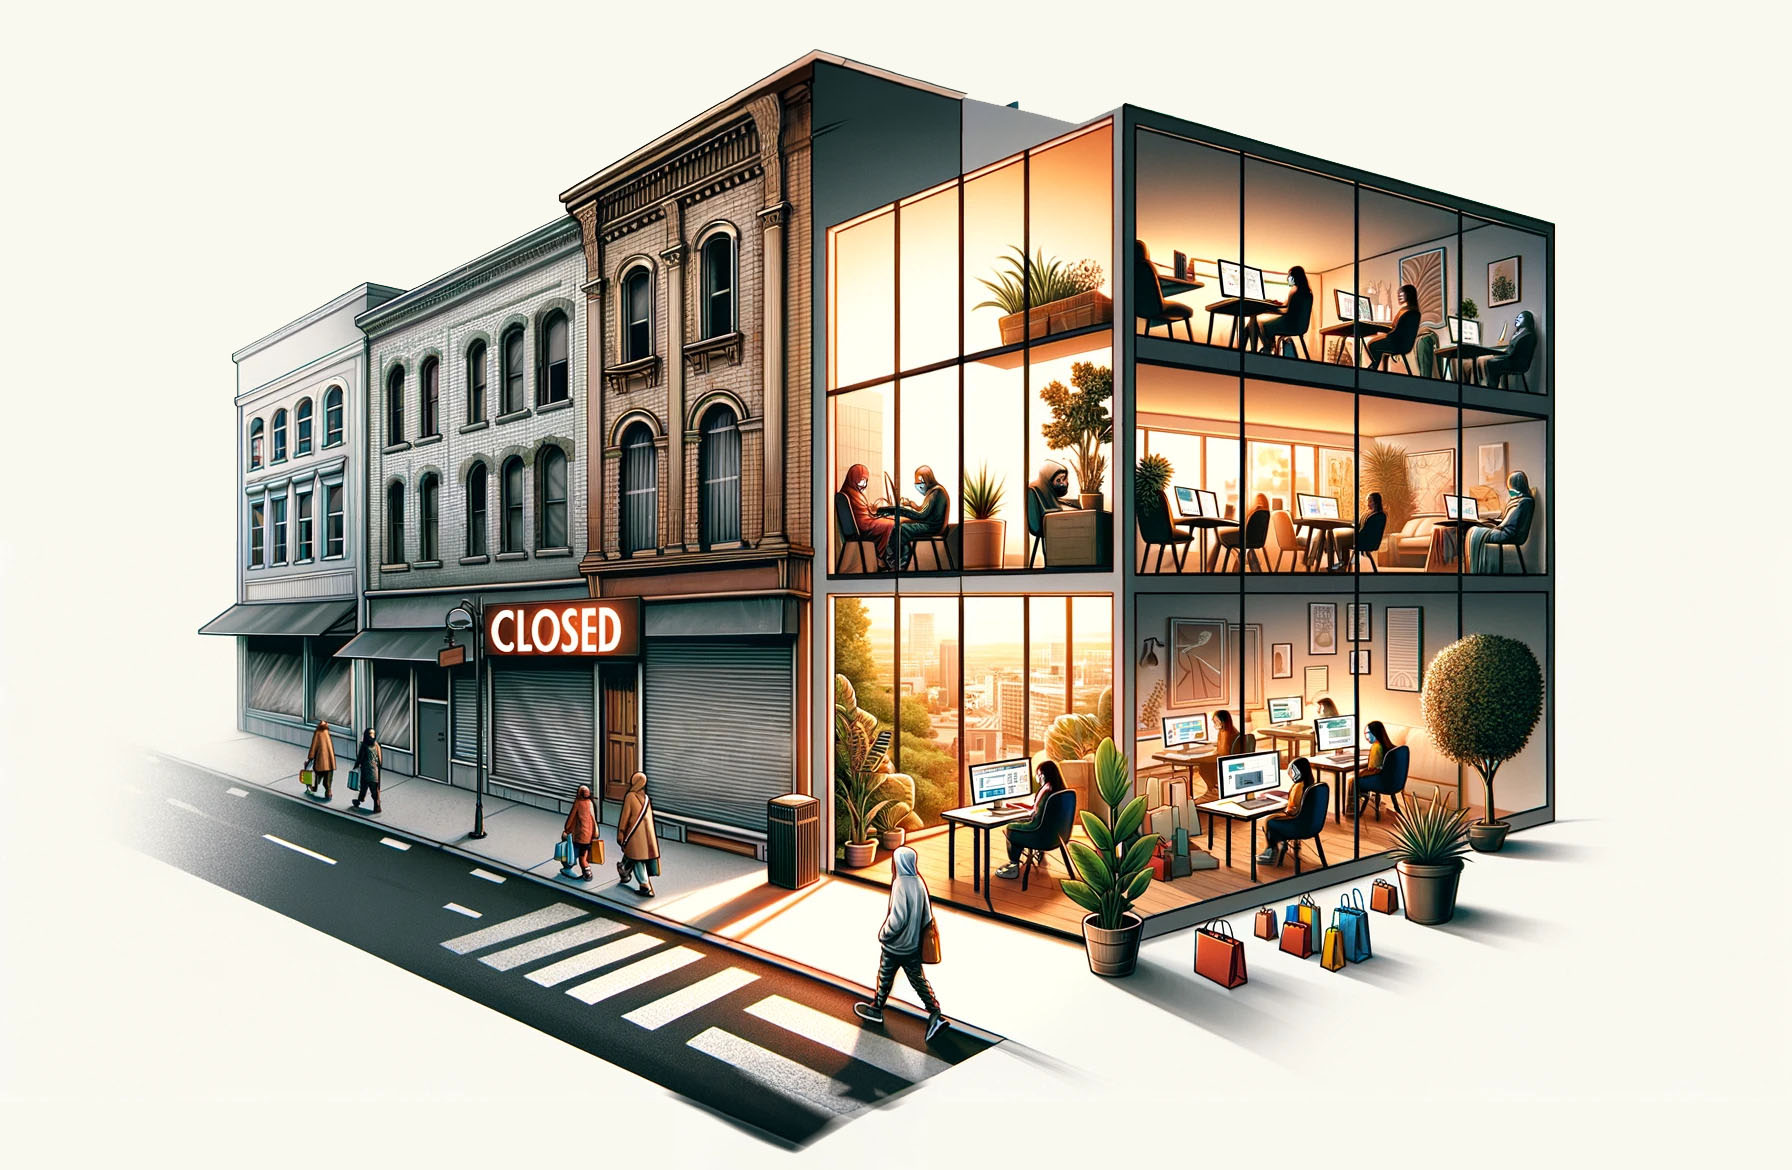
\includegraphics[width=0.9\linewidth]{figure/art2.jpg}
\end{figure}

% Cover text
\mbox{}
\vfill
\renewcommand{\familydefault}{\sfdefault} \normalfont % Set cover page font
\textbf{{\Huge 	\subject 	\\[0.2cm] }} 	\\[0.5cm]

{\small \maintitle \\[0.2cm]}
    
% {\Large A Subtitle that can be Very Much Longer if Necessary}\\[0.5cm]
% Master's thesis in Master Programme Name \setlength{\parskip}{1cm}

\noindent
{\Large \authorm \\[0.18cm]
\authorp \\[0.1cm]
\authort
} \setlength{\parskip}{1.5cm}

\noindent
\textcolor{thesisHeaderColor}{\small\textbf{\textsc{\dept}}}
\setlength{\parskip}{1mm}

\textsc{\university} \\
{\small \address \the\year \\
\href{\site}{\site}}\vspace{1.7cm}

\renewcommand{\familydefault}{\rmdefault} \normalfont % Reset standard font
\end{titlepage}


% BACK OF COVER PAGE (BLANK PAGE)
\newpage
\restoregeometry
\thispagestyle{empty}
\mbox{}


% TITLE PAGE
\newpage
\thispagestyle{empty}
\begin{center}
	\textsc{\large \subject \the\year}\\[4cm]
	\textbf{\Large \maintitle} \\[1cm]
	% {\large A Subtitle that can be Very Much Longer if Necessary}\\[1cm]
	{\large \authorm} \\[0.1cm]
        {\large \authorp} \\[0.1cm]
        {\large \authort}
	
	\vfill	
	% Logotype on titlepage	
	\begin{figure}[H]
	\centering
	% Remove this figure to remove the titlepage logotype
	\if\ThesisType M
    
\includegraphics[width=0.2\pdfpagewidth]{figure/auxiliary/logo_circle.png} \\
    \fi
    \if\ThesisType B
    
\includegraphics[width=0.2\pdfpagewidth]{figure/auxiliary/logo_circle.png} \\
    \fi

	\end{figure}	\vspace{5mm}	
	
	\dept \\
	% \emph{Division of Division name}\\
	% Name of research group (if applicable)\\
	\textsc{\university} \\
	\address \  \the\year \\
\end{center}


% IMPRINT PAGE (BACK OF TITLE PAGE)
\newpage
\thispagestyle{plain}
\vspace*{4.5cm}
\maintitle \\
% A Subtitle that can be Very Much Longer if Necessary\\
\\[0.1cm]
\authorm \\
\authorp \\
\authort
\setlength{\parskip}{1cm}

% \copyright ~ NAME FAMILYNAME, \the\year. \setlength{\parskip}{1cm}

Supervisor: \supervisor \\
Examiner: \examiner \setlength{\parskip}{1cm}

\subject \\	
\dept \\
% Division of Division name\\
% Name of research group (if applicable)\\
\university \\
\address \\
% Telephone +46 31 772 1000 
\setlength{\parskip}{0.5cm}

\vfill
% Caption for cover page figure if used, possibly with reference to further information in the report
Cover - \textbf{Contrast in Commerce:} A Generative Image of Closed Shops and Bustling Online Markets. \setlength{\parskip}{0.5cm}

Typeset in \LaTeX \tagtemp\\
Printed by XXX \\
\address \ \the\year
